\lecture{Эффективные методы построения фигур}{Темерлан Ахметов}

\subsection{Отрисовка окружности}

\textbf{Растеризация} — это ключевой этап компьютерной графики, где геометрические формы, заданные в непрерывных координатах (например, линии, окружности, многоугольники), преобразуются в набор пикселей на экране. Экран представляет собой дискретную сетку, поэтому для отображения объектов требуется выбрать конкретные пиксели, которые лучше всего приближаются к математическим фигурам.

\textbf{Основные задачи растеризации:}
\begin{enumerate}
    \item \textbf{Приведение к дискретной форме}: Компьютерные экраны состоят из сетки пикселей, а фигуры — из непрерывных линий. Растеризация определяет, какие пиксели нужно "зажечь", чтобы фигура была максимально точной.
    \item \textbf{Оптимизация}: Современные приложения требуют высокой скорости обработки, поэтому растеризация должна быть вычислительно дешёвой.
    \item \textbf{Унификация}: Любая фигура (окружность, линия, многоугольник) может быть растеризована с использованием общих подходов.
\end{enumerate}

\paragraph*{Проблема расчёта окружности}
Для рисования окружности требуется удовлетворять уравнению окружности:

\[
    x^2 + y^2 = R^2
\]

Но при вычислении координат возникают сложности:

\begin{enumerate}
    \item $y = \sqrt{R^2-x^2}$: требует вычисления квадратного корня, что вычислительно дорого.
    \item $y = R sin(\alpha)$: требует вычисления тригонометрических функций. Можно ускорить с помощью таблиц, но всё равно есть ограничения.
\end{enumerate}

\textbf{Идея}: вместо пересчёта каждой точки окружности, использовать свойства симметрии окружности и дискретный подход, подобный алгоритму \textbf{Брезенхейма}.

\begin{itemize}
    \item Окружность обладает 8-кратной симметрией (отражение по осям и диагоналям). Поэтому достаточно рассчитать одну восьмую часть окружности (восьмушку) и отразить её на остальные части.
    \item Это сокращает количество расчётов в 8 раз.
\end{itemize}

\subsubsection*{Алгоритм Брезенхэма}
Алгоритм Брезенхэма — один из самых эффективных методов для растеризации окружностей.

Алгоритм работает на основе анализа текущей ошибки $D$, которая показывает, насколько точка отклоняется от истинной окружности.

$(x_l, y_l)$ -- текущая точка на сетке, которую уже выбрали как часть окружности.
Из этой точки нужно выбрать следующий пиксель, который лучше всего приближает окружность.

Для текущей точки $P_l = (x_l, y_l)$
\begin{itemize}
    \item $D(P_l) = (x_l^2 + y_l^2) - R^2$: показывает отклонение от окружности.
    \item Есть два варианта следующей точки:
          \begin{enumerate}
              \item Точка \textbf{справа}: $S_l = (x_l + 1, y_l)$.
              \item Точка \textbf{справа и ниже}: $T_l = (x_l + 1, y_l - 1)$
          \end{enumerate}
\end{itemize}

Для выбора следующей точки:
\begin{itemize}
    \item Считается ошибка для каждой точки:
          \begin{itemize}
              \item $D(S_l) = ((x_l + 1)^2 + y_l^2) - R^2$ -- ошибка точки выше.
              \item $D(T_l) = ((x_l + 1)^2 + (y_l - 1)^2) - R^2$ -- ошибка точки ниже.
          \end{itemize}
    \item Выбирается точка с меньшей ошибкой:
          \begin{itemize}
              \item Если $|D(S_l)| < |D(T_l)$, рисуется $S_l$.
              \item Если $|D(S_l)| > |D(T_l)$, рисуется $T_l$.
              \item Если ошибки равны, можно выбрать любую.
          \end{itemize}
\end{itemize}

\begin{figure}[H]
    \centering
    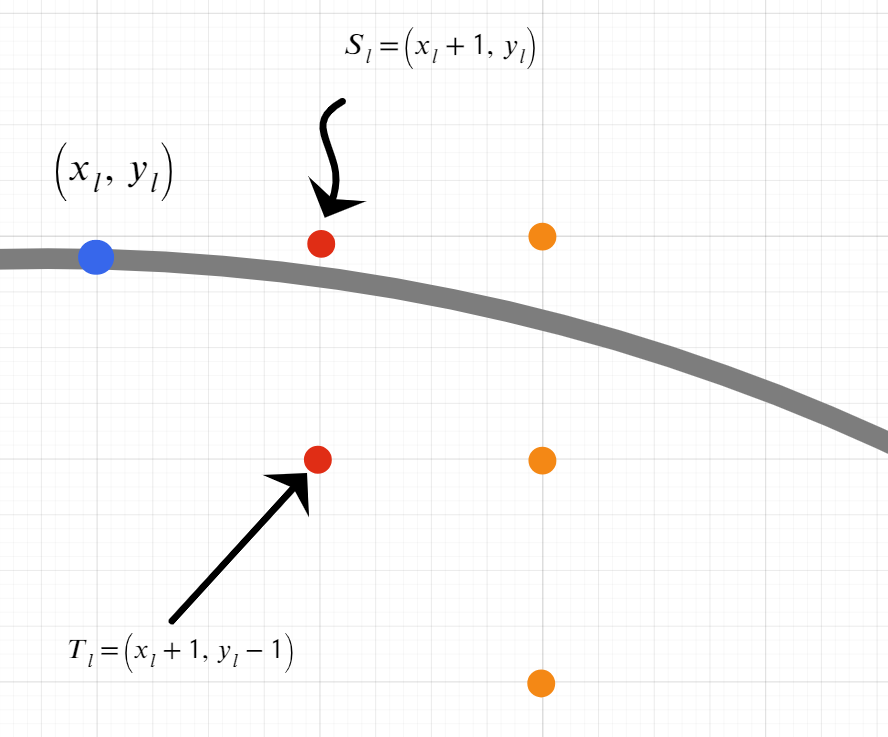
\includegraphics[width=0.6\linewidth]{example.png}
    \caption{Выбор следующего пикселя}
    \label{fig:next_pixel}
\end{figure}

На рисунке \ref{fig:next_pixel}:
\begin{itemize}
    \item Синяя точка \((x_l, y_l)\) — текущий пиксель.
    \item Красные точки \( S_l \) и \( T_l \) — варианты следующего пикселя.
    \item Оранжевые точки — возможные последующие пиксели.
\end{itemize}

\subsubsection*{Оптимизация c расчётом ошибки}
Вместо пересчёта ошибок с нуля, используются разности между текущими и следующими точками:

\begin{itemize}
    \item Если выбрана точка $S_l$:
          \[
              d_{l+1} = d_l + 4x_l + 6
          \]
    \item Если выбрана точка $T_l$:
          \[
              d_{l+1} = d_l + 4(x_l - x_y) + 10
          \]
\end{itemize}
Эти формулы позволяют эффективно обновлять ошибки и выбирать следующую точку без повторных вычислений.

\subsubsection*{Критерий завершения} Алгоритм проходит по точкам, начиная с верхней точки окружности $(0, R)$, и заканчивает, когда $x\geq y$. Это происходит из-за симметрии окружности.
\begin{figure}[H]
    \centering
    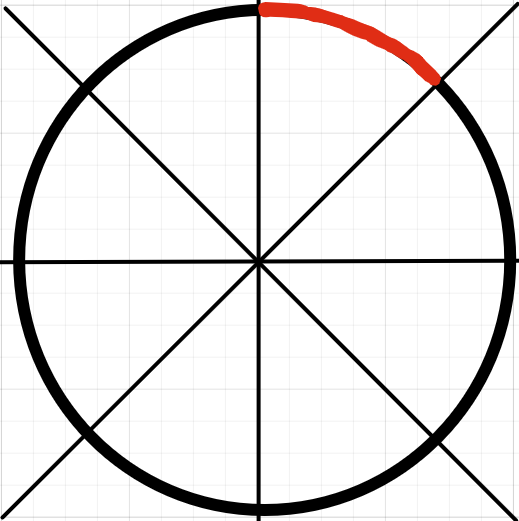
\includegraphics[width=0.5\linewidth]{circle0.25.png}
    \caption{Заполненная $1/8$}
    \label{fig:circle_0.25}
\end{figure}

После завершения восьмой части (восьмушки), эта информация может быть отражена на остальных частях окружности (за счёт симметрии):
\begin{itemize}
    \item Нужно отразить точки на оставшиеся 7 частей окружности.
\end{itemize}

\begin{figure}[H]
    \centering
    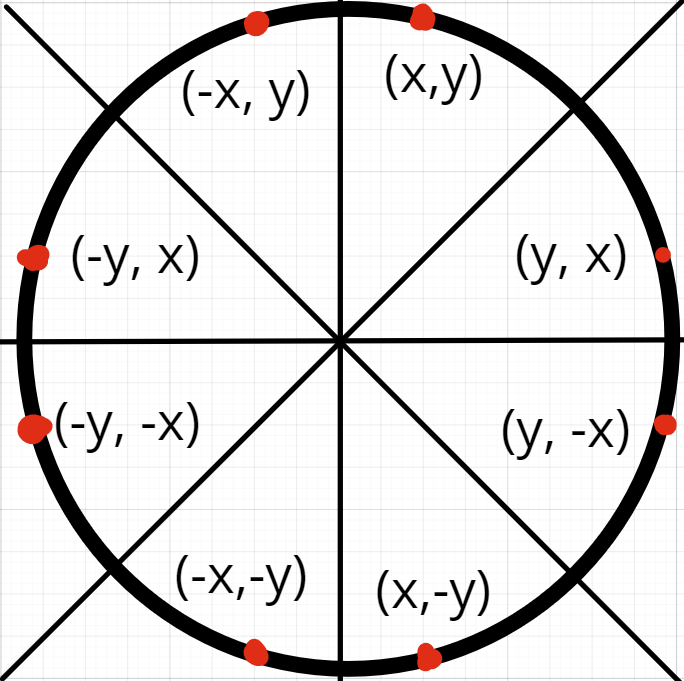
\includegraphics[width=0.5\linewidth]{circle.png}
    \caption{Симметричные точки}
    \label{fig:circle}
\end{figure}

\subsection{Задача заполнения цветами (Алгоритм Сазерленда–Ходжмена)}
Алгоритм Сазерленда–Ходжмена используется для отсечения многоугольника, часть которого выходит за пределы окна.

\subsubsection*{Зачем необходимо отсечение?}
При визуализации сцены на экране часть многоугольника может выходить за границы видимой области (окна). Затраты на закрашивание невидимых частей кадра неэффективны, так как они не будут отображаться пользователю. Поэтому на этапе заполнения цветом выполняется предварительное отсечение: прямоугольное окно ограничивает область обработки, и из многоугольника удаляются лишние части.

\subsubsection*{Алгоритм}
Рассматривается задача заполнения многоугольника цветом, ограниченного заданным окном.  \\
Многоугольник состоит из вершин:
$P_1, P_2 \dots P_n$, где \( P_i \rightarrow P_{i+1} \), а \( P_n \rightarrow P_1 \).\\
$B_1B_2B_3B_4$ -- заданное прямоугольное окно

Принцип работы:
\begin{itemize}
    \item Каждая граница окна рассматривается как бесконечно продолженная линия, которая делит пространство на две части: внутреннюю (в пределах окна) и внешнюю (за пределами окна).
    \item Обработка многоугольника осуществляется по каждой границе окна последовательно.
\end{itemize}

Шаги алгоритма: Для каждой границы выполняются следующие действия:
\begin{enumerate}
    \item Проверка каждого ребра $P_i \rightarrow P_{i+1}$
          \begin{itemize}
              \item Если обе вершины рёбра находятся внутри окна, ребро сохраняется.
              \item Если одно из концов рёбра находится снаружи, вычисляется точка пересечения рёбра с текущей границей. Новая точка добавляется в список вершин.
              \item Если оба конца рёбра находятся снаружи, ребро отбрасывается.
          \end{itemize}
    \item Полученный многоугольник передаётся для обработки следующей границы.
\end{enumerate}
\begin{figure}[H]
    \centering
    % Первая пара изображений
    \begin{subfigure}[b]{0.5\linewidth}
        \centering
        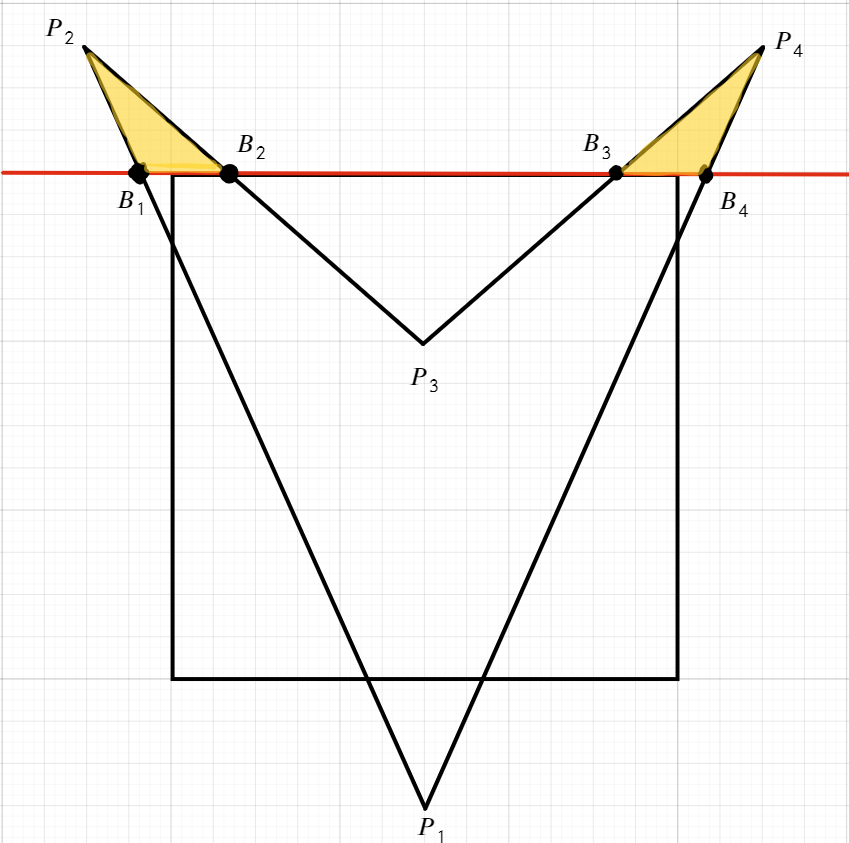
\includegraphics[width=\linewidth]{screen_1.png}
        \caption{Итерация 1}
        \label{fig:iter1}
    \end{subfigure}
    \hfill
    \begin{subfigure}[b]{0.45\linewidth}
        \centering
        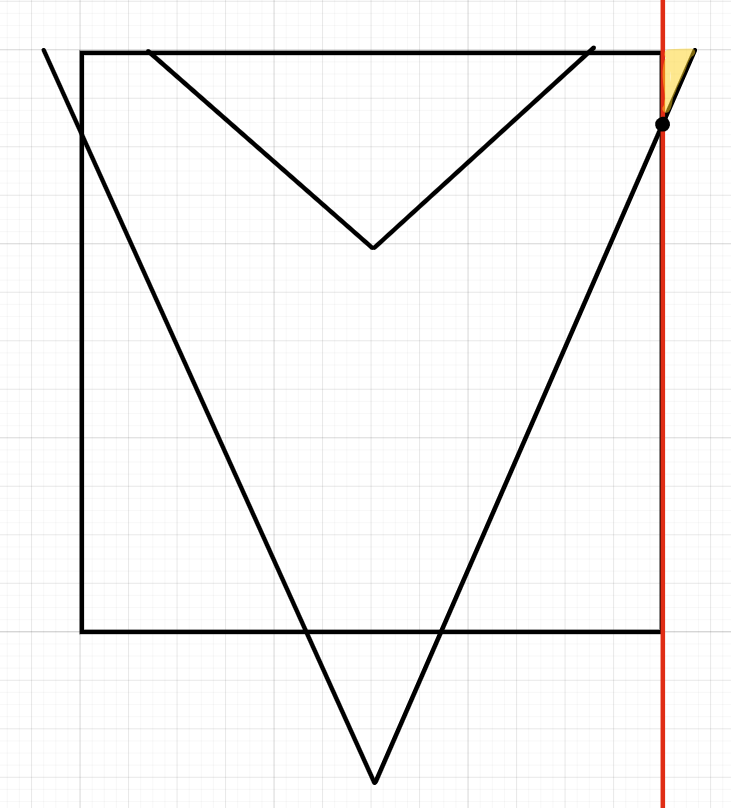
\includegraphics[width=\linewidth]{screen_2.png}
        \caption{Итерация 2}
        \label{fig:iter2}
    \end{subfigure}
    \caption{}
    \label{fig:pair_iter1_iter2}
\end{figure}

\begin{figure}[H]
    \centering
    % Вторая пара изображений
    \begin{subfigure}[b]{0.425\linewidth}
        \centering
        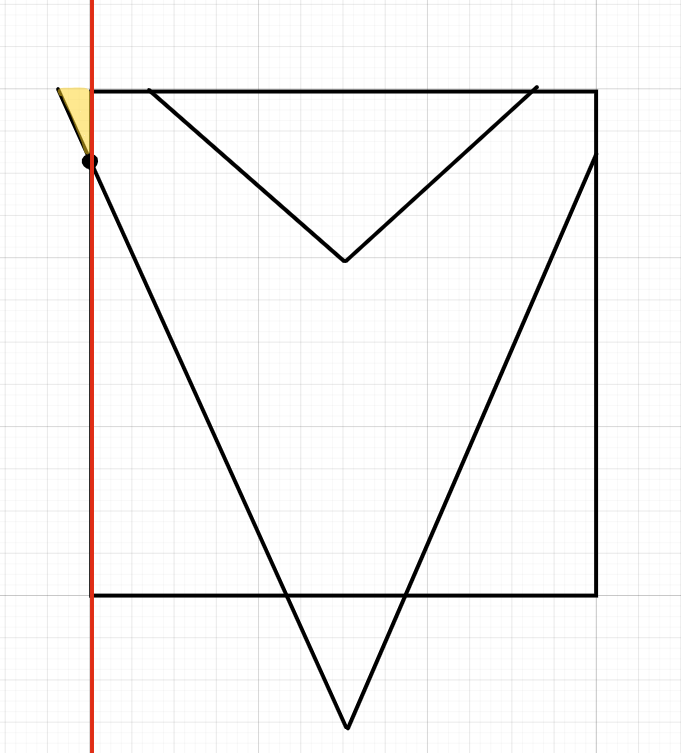
\includegraphics[width=\linewidth]{screen_3.png}
        \caption{Итерация 3}
        \label{fig:iter3}
    \end{subfigure}
    \hfill
    \begin{subfigure}[b]{0.5\linewidth}
        \centering
        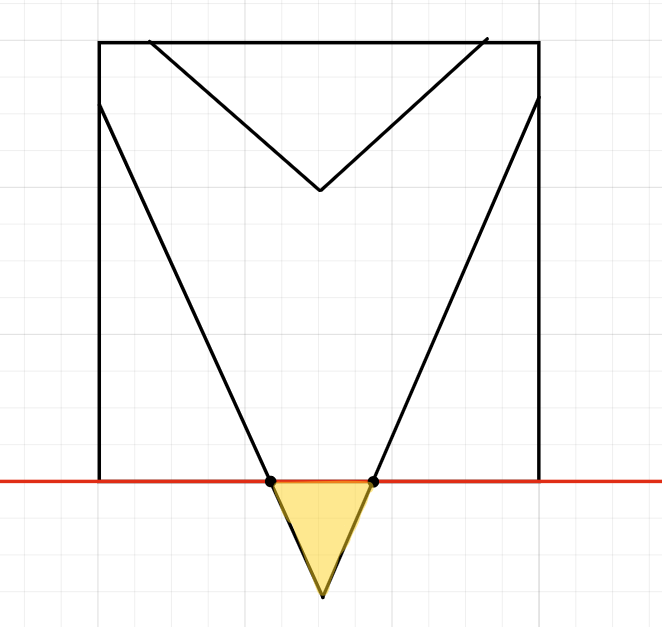
\includegraphics[width=\linewidth]{screen_4.png}
        \caption{Итерация 4}
        \label{fig:iter4}
    \end{subfigure}
    \caption{}
    \label{fig:pair_iter3_iter4}
\end{figure}

\textbf{Результат}: После прохождения всех четырёх границ окна формируется новый многоугольник, состоящий из вершин, которые полностью находятся внутри окна.

\begin{figure}[H]
    \centering
    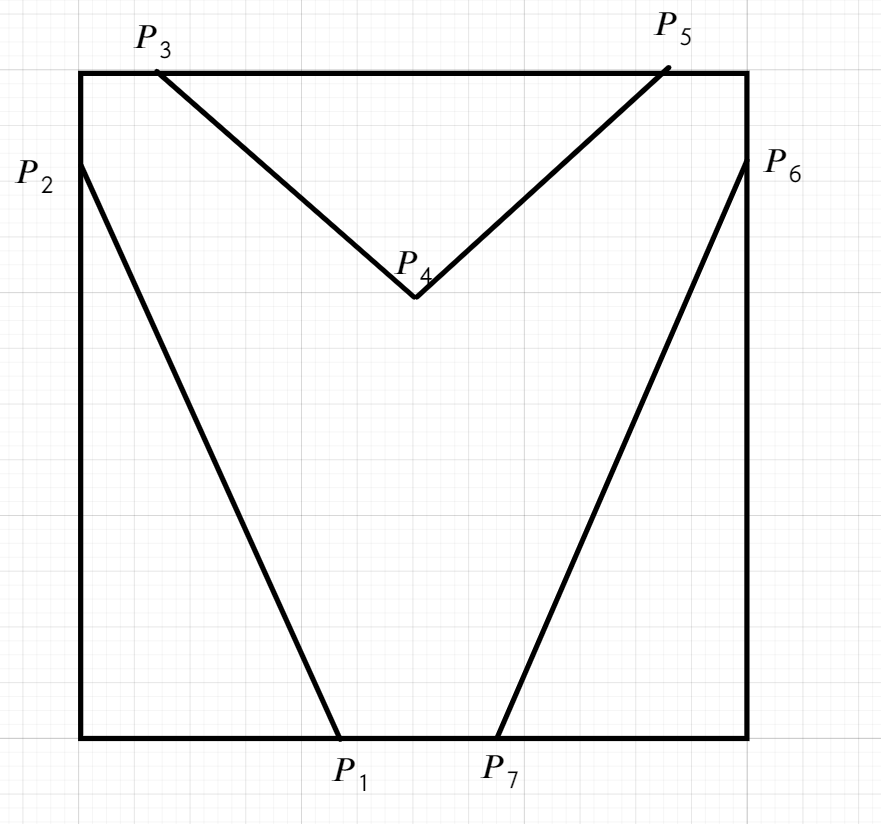
\includegraphics[width=0.5\linewidth]{final.png}
    \caption{Результат}
    \label{fig:final}
\end{figure}

